\section{Auswertung}
\label{sec:Auswertung}

Alle Berechnungen werden mit dem Programm \glqq Numpy" \cite{numpy}, die Unsicherheiten mit dem Modul \glqq Uncertainties" \cite{uncertainties}, die Ausgleichsrechnungen mit dem Modul \glqq Scipy" \cite{scipy} durchgeführt und die grafischen Darstellungen über das Modul \glqq Matplotlib" \cite{matplotlib} erstellt.
In der Auswertung wird mit logarithmischen Fehlern gerechnet, welche bei einem nicht logarithmischen Fehler $\Delta N$ aus einer Abweichung nach Oben und nach Unten wie foolgt zusammensetzten:
\begin{align*}
    \Delta^{+} \ln (N)&=\ln (N+\Delta N)-\ln (N) \\
    \Delta^{-} \ln (N)&=\ln (N)-\ln (N-\Delta N)
\end{align*}

\subsection{Untergrundrate}

Aus dem mehrfachen Messen der Untergrundrate ergeben sich die Messwerte $N_U=\{ 129, 143, 144, 136, 139, 126, 158 \}$. Aus diesen Messwerten wird der Mittelwert berechnet. Dieser ergibt sich zu $\num{139(4)}$. Da die Zeit, über die die Impulse gemessen werden, mit den Messintervallen der folgenden Messergebnisse übereinstimmen muss, wird  dieser Mittelwert auf die jeweiligen Messintervalle skaliert. So ergibt sich eine Untergrundrate von $N_{U_V}=\num{14(1)}$ in einem Zeitintervall von $\Delta t=\SI{30}{\s}$ und $N_{U_R}=\num{7(1)}$ in einem Zeitintervall von $\Delta t=\SI{15}{\s}$.

\subsection{Halbwertszeit Vanadium}
\label{Vanadium}

Die gemessenen Impulse sind in Tablle \ref{tab:V} aufgeführt. Da die Werte poissonverteilt sind, berechnet sich der Fehler über $\Delta N=\sqrt{N}$. Von den gemessenen Impulsen muss jeweils die Untergrundrate $N_{U_R}$ abgezogen werden. Die dadurch bestimmten Impulsraten sind grafisch in einem Halblogarithmischen Diagramm \ref{fig:V} dargestellt. Über \eqref{eqn:N} lässt sich ein linearer Zusammenhang zwischen $\ln{N}$ und der Zerfallskonstante $\lambda $ feststellen. Wird also eine lineare Regression durchgeführt, so ergibt sich eine Gerade
\begin{equation}
    \ln{N}(t)=at + b
    \label{eqn:gerade}
\end{equation}
mit den Geradenparametern $a_V=\SI[per-mode=reciprocal]{-0.0323(00011)}{\per\s}$ und $b_V=\num{5.32(04)}$. 
Aus der Steigung $a$ kann die Zerfallskonstante $\lambda$ über
\begin{equation}
    \lambda=-a
\label{eqn:lamb}
\end{equation}
berechnet werden. Mit dem $\lambda_V$ ergibt sich dann über \eqref{eqn:T} eine Halbwertszeit von 
${T_V=\SI{215(7)}{\s}}$.


\begin{table}
\caption{Anzahl registrierter Impulse der Vanadium-Probe.}
\centering
\label{tab:V}
\sisetup{table-format=4}
\begin{tabular}{S S}
\toprule
{$t \:/\: \si{\s}$} & {$N$} \\

\midrule
30	 & \num{189(14)} \\
60	 & \num{197(14)} \\
90	 & \num{150(12)} \\
120	 & \num{159(13)} \\
150	 & \num{155(12)} \\
180	 & \num{132(11)} \\
210	 & \num{117(11)} \\
240	 & \num{107(10)} \\
270	 & \num{94( 19)} \\
300	 & \num{100(10)} \\
330	 & \num{79( 9 )} \\
360	 & \num{69( 8 )} \\
390	 & \num{81( 9 )} \\
420	 & \num{46( 7 )} \\
450	 & \num{49( 7 )} \\
480	 & \num{61( 8 )} \\
510	 & \num{56( 7 )} \\
540	 & \num{40( 6 )} \\
570	 & \num{45( 7 )} \\
600	 & \num{32( 6 )} \\
630	 & \num{27( 5 )} \\
660	 & \num{43( 7 )} \\
\bottomrule
\end{tabular}
\begin{tabular}{S S}
\toprule
{$t \:/\: \si{\s}$} & {$N$} \\

\midrule
690	 & \num{35( 6 )} \\
720	 & \num{19( 4 )} \\
750	 & \num{28( 5 )} \\
780	 & \num{27( 5 )} \\
810	 & \num{36( 6 )} \\
840	 & \num{25( 5 )} \\
870	 & \num{29( 5 )} \\
900	 & \num{18( 4 )} \\
930	 & \num{17( 4 )} \\
960	 & \num{24( 5 )} \\
990	 & \num{21( 5 )} \\
1020 & \num{25( 5 )} \\
1050 & \num{21( 5 )} \\
1080 & \num{24( 5 )} \\
1110 & \num{25( 5 )} \\
1140 & \num{17( 4 )} \\
1170 & \num{20( 4 )} \\
1200 & \num{19( 4 )} \\
1230 & \num{20( 4 )} \\
1260 & \num{18( 4 )} \\
1290 & \num{16( 4 )} \\
1320 & \num{17( 4 )} \\


\bottomrule

\end{tabular}
\end{table}

\begin{figure}
\centering
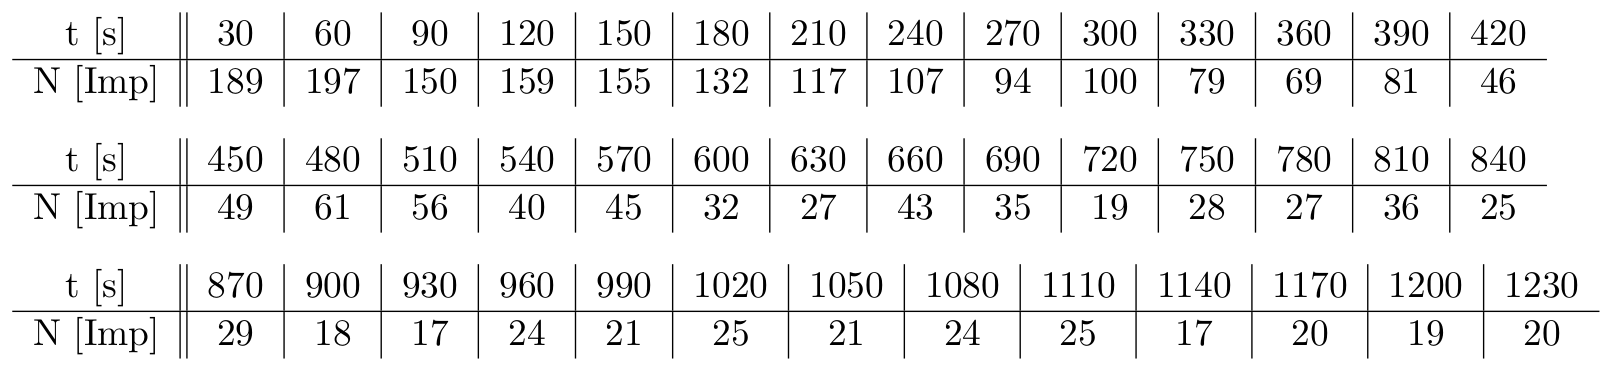
\includegraphics{build/Vanadium.pdf}
\caption{Bereinigte Messdaten und Ausgleichsgerade von Vanadium.}
\label{fig:V}
\end{figure}

\subsection{Halbwertszeit Rhodium}
\label{Rhodium}
Beim Zerfall von Rhodium müssen die beiden überlagerten Zerfälle getrennt analysiert werden. Die Messdaten sind in Tabelle \ref{tab:R} aufgeführt. Werden die vom Untergrund bereinigten Impulse grafisch dargestellt (Abbildung \ref{fig:R}), lässt sich der Bereich, in dem nur noch der langsame Zerfall stattfindet, identifizieren. Ab $t=\SI{255}{\s}$ kommen beinahe keine Zerfälle von $\ce{^{104i}Rh}$ mehr vor. In die nachfolgenden Werte wird eine Ausgleichsgerade gelegt und durch Extrapolation die Impulsanteile des langsamen Zerfalls im Bereich $t\leq\SI{210}{\s}$ bestimmt. Diese werden von den Impulsen in diesem Bereich abgezogen und es werden die von dem langsamen Zerfall bereinigten Impulse des schnellen Zerfalls erhalten. Durch diese Werte wird ebenfalls eine Ausgleichsgerade gelegt. Dabei wird der Übergangsbereich $t=\SI{210}{\s}-\SI{270}{\s}$ zwischen schnellem und langsamen Zerfall aus der lineareen Regression entfernt, sodass die beiden Bereiche klarer getrennt sind. Aus den beiden Geraden, die wieder die Form \eqref{eqn:gerade} haben, können die Geradenparameter des schnellen Zerfalls zu 
\begin{align*}
a_{R_s} & = \SI{-0.0161(0004)}{\frac{1}{\s}} \;\text{und}  \\
b_{R_s} & = \num{6.678(025)}
\end{align*}
bestimmt werden. Die Geradenparameter des langsamen Zerfalls ergeben sich zu 
\begin{align*}
a_{R_l} & =\SI{-0.0027(0004)}{\frac{1}{\s}} \;\text{und} \\ 
b_{R_l} & =\num{4.35(17)}.
\end{align*} 
Über \eqref{eqn:lamb} kann wieder die jeweilige Zerfallskonstante
\begin{align*}
 \lambda_{R_s} & = \SI{0.0161(0004)}{\frac{1}{s}}  \; \text{und}\\
 \lambda_{R_l} & = \SI{0.0027(0004)}{\frac{1}{s}}
 \end{align*}
 bestimmt werden. Aus diesen Zerfallskonstanten lässt sich über \eqref{eqn:T} die Halbwertszeit von $\ce{^{104i}Rh}$ zu $T_{R_l}=\SI{260(40)}{\s}$ und die Halbwertszeit von $\ce{^{104}Rh}$ zu $T_{R_s}=\SI{43.0(11)}{\s}$ bestimmen.



\begin{table}
\centering
\caption{Anzahl registrierter Impulse der Rhodium-Probe.}
\label{tab:R}
\sisetup{table-format=4}
\begin{tabular}{S S}
\toprule
{$t \:/\: \si{\s}$} & {$N$} \\

\midrule

15	 & \num{667(26 )}  \\
30	 & \num{585(24) } \\	 
45	 & \num{474(22 )}  \\
60	 & \num{399(20) } \\
75	 & \num{304(17 )}  \\
90	 & \num{253(16) } \\
105	 & \num{213(15) } \\
120	 & \num{173(13 )}  \\
135	 & \num{152(12) } \\
150	 & \num{126(11) } \\
165	 & \num{111(11 )}  \\
180	 & \num{ 92(10) } \\
195	 & \num{ 79(9)  }\\
210	 & \num{ 74(7)  }\\
225	 & \num{ 60(8)  }\\
240	 & \num{ 52(7 ) } \\
255	 & \num{ 56(7)  }\\
270	 & \num{ 53(7)  }\\
285	 & \num{ 41(6)  }\\
300	 & \num{ 36(6)  }\\
315	 & \num{ 37(6 ) } \\
330	 & \num{ 32(6  )}  \\
\bottomrule
\end{tabular}
\begin{tabular}{S S}
\toprule
{$t \:/\: \si{\s}$} & {$N$} \\

\midrule
345	 & \num{ 36(6)  }\\
360	 & \num{ 38(6)  }\\
375	 & \num{ 34(6  )}  \\
390	 & \num{ 40(6  )}  \\
405	 & \num{ 21(5  )}  \\
420	 & \num{ 35(6 ) } \\
435	 & \num{ 33(6  )}  \\
450	 & \num{ 36(6)  }\\
465	 & \num{ 20(4 ) } \\
480	 & \num{ 24(5)  }\\
495	 & \num{ 30(5 ) } \\
510	 & \num{ 30(5  )}  \\
525	 & \num{ 26(5  )}  \\
540	 & \num{ 28(5)  }\\
555	 & \num{ 23(5  )}  \\
570	 & \num{ 20(4  )}  \\
585	 & \num{ 28(5  )}  \\
600	 & \num{ 17(4 ) } \\
615	 & \num{ 26(5 ) } \\
630	 & \num{ 19(4)  } \\
645	 & \num{ 13(4 ) } \\
660	 & \num{ 17(4)  } \\

\bottomrule

\end{tabular}
\end{table}

\begin{figure}
\centering
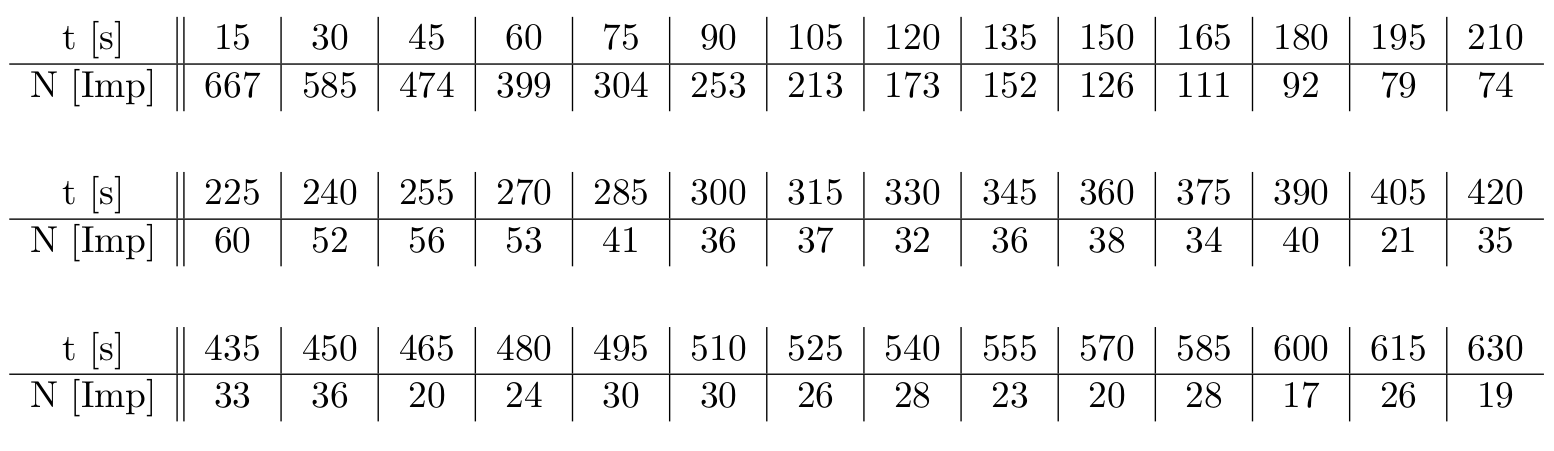
\includegraphics{build/Rhodium.pdf}
\caption{Bereinigte Messdaten und Ausgleichsgeraden von Rhodium.}
\label{fig:R}

\end{figure}


%Messwerte: Alle gemessenen physikalischen Größen sind übersichtlich darzustellen.
%
%Auswertung:
%Berechnung der geforderten Endergebnisse
%mit allen Zwischenrechnungen und Fehlerformeln, sodass die Rechnung nachvollziehbar ist.
%Eine kurze Erläuterung der Rechnungen (z.B. verwendete Programme)
%Graphische Darstellung der Ergebnisse